\documentclass[main.tex]{subfiles}

\begin{document}

\section{Adaptive Software Development}

Adaptive software development (ASD) is an iterative, circular process of software development created by \textbf{Jim Highsmith} and \textbf{Sam Bayer}. It is a methodology for building complex software applications and systems published in 2000.

ASD is characterized by a rapid creation and evolution of the software application with an emphasis on collaboration. It is a successor to rapid application development and a predecessor of modern agile development techniques.\supercite{adaptive-wikidot,adaptive-wikipedia}

ASD derives its conceptual perspective from the Complex Adaptive Systems (CAS) theory --- from which it inherits its Emergence and Complexity --- and its practical perspective on the Rapid Application Development techniques and deterministic methodologies.

The ASD cycle has six basic characteristics:\supercite{adaptive-ecosystems}
\begin{enumerate}
	\item Mission focused
	\item Feature based
	\item Iterative
	\item Time-boxed
	\item Risk driven
	\item Change tolerant
\end{enumerate}

\subsection{The Process of Adaptive Software Development}

\begin{wrapfigure}[16]{l}[2em]{0.6\textwidth}
	\vspace*{-\baselineskip}
	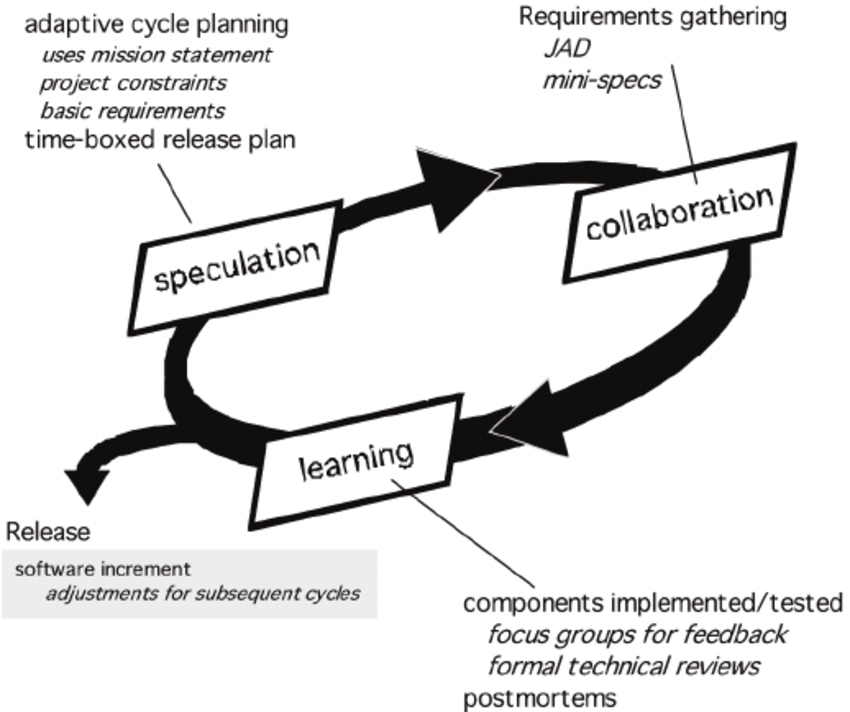
\includegraphics[scale=0.3]{adaptive-cycle.png}
	\caption{The Adaptive cycle\label{fig:adaptive-cycle}}
\end{wrapfigure}

Adaptive replaces the traditional linear waterfall model with a repeating series of \emph{speculate}, \emph{collaborate} and \emph{learn} cycles.
It is characterized by constant change, re-evaluation, peering into an uncertain future and intense collaboration among developers, testers and customers in the various phases.

\subsubsection[Speculation]{1. Speculation}

This is the setup phase. During it, developers attempt to understand the exact nature of the product's requirements --- what features need to be added, what problems need to be fixed, and what changes need to be made.

To facilitate this, a previous cycle feeds information to this phase, namely bugs, user reports, new requirements found during developments and finished or unfinished features.

Let's see how \emph{speculation} comprises \emph{project initiation} and \emph{cycle planning}.

\paragraph{Project Initiation} The project's constraints and \textit{mission statement} are set by the customer. The development team determines the project's organization, gathers more requirements, and estimates size and scope.

% The \emph{mission statement} needs to be specific, yet flexible. Attempting to excel in multiple dimensions usually results in a product being mediocre in all of them and excellent in none, or delayed releases.

\paragraph{Cycle Planning} The mission statement's aim is to expose the customer's desired result for the project.
It's likely that the customer has no knowledge of the field, so this can be done adequately in layman's terms. Using the mission statement, the team forces it's focus on a single area --- such as features, schedule, defects, or resources --- in which it must excel in the development phase. This is inherently risk-driven: attempting to excel in all dimensions usually results in a product being mediocre in all of them and excellent in none (or delayed releases), so compromises must be made.

Finally, the team fixes a set of features to implement in the next iteration and also \emph{fixes} a certain amount of time for it.

\subsubsection[Collaboration]{2. Collaboration}

This is the development phase. Here, effective collaboration within the team is key. Complex applications are not built --- they evolve. In this high information flow environment, one person or small group can't possibly \textsl{know it all}, so collaboration skills are paramount.

Collaboration and communication with the client continues, but only to handle minor issues/requirements adjustments and preference resolutions.

\subsubsection[Learning]{3. Learning}

This is the quality control phase. Here is where many integration and system tests are performed. Knowledge is gathered about the project's state to prepare for the next speculation phase.

Focus groups, technical reviews and project artifacts are characteristic of this phase. Giving a status report to the customer and receiving feedback is the common goal. In a focus group, the application or system being developed is presented to the customer, who then gives feedback, records change requests, and helps prepare a mission statement.

Summing up, there are four aspects to report on at the end of each iteration:

\begin{itemize}
	\item Result quality from the customer's perspective.
	\item Result quality from a technical perspective.
	\item The functioning of the delivery team and the practices team members are utilizing.
	\item The project's status.
\end{itemize}

\subsection{Artifacts}

\paragraph{Project Vision}
A document which serves to establish a focus for the project,\supercite{adaptive-collaborative} and identifies the foundation on which to build the team's commitment.
It should help developers explain the project's purpose within a few minutes. The document may include: Project Background; Project Scope; Sponsors; Customers; Business Functional Objectives; Project Risks; Staffing Requirements; Constraints; Assumption...

\paragraph{Project Data Sheet}
A document which results from a project initiation. Includes: client, project objective statement, features, performance or quality attributes, architecture, issues and risks, milestones, and the team's core members.

\begin{wrapfigure}[8]{r}[2em]{0.4\textwidth}
	\vspace*{-\baselineskip}
	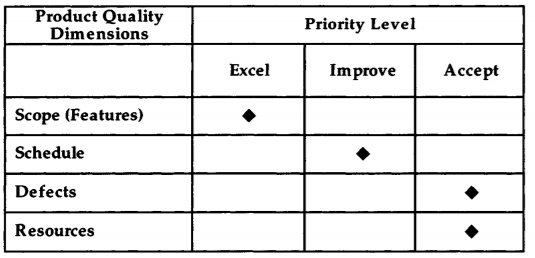
\includegraphics[scale=0.35]{adaptive-mission-matrix.png}
	\caption{Mission Profile's Matrix\label{fig:mission-matrix}}
\end{wrapfigure}

\paragraph{Product Mission Profile}
A short document used to record focus for the next development iteration, using for instance profile matrices (\autoref{fig:mission-matrix}). These may be done per iteration or per feature.\supercite{adaptive-collaborative}
In the example, the \textsl{Excel} column identifies Scope as the most important dimension for the next iteration.

\paragraph{Project Specification Outline}
It serves several purposes.
First, it provides the stakeholders and team members with a reasonable understanding of the boundaries and scope of the development effort.
Second, it is a baseline for size estimation.
Finally, the PSO facilitates adaptive cycle planning and is accomplished by assigning product features to specific cycles.
The specification outline's primary objective is to define the features or functionality of the product.\supercite{adaptive-collaborative}

\subsection{Pros and Cons}

\paragraph{Pros}
\begin{itemize}
	\item Allows for transparency because developers explain the state of the project to the client before, during and after each stage;
	\item Generates high quality software, breaking down the project into components, concentrating on high quality development, testing of one component at a time, aids in producing a high quality end product in the end run.
\end{itemize}

\paragraph{Cons}
\begin{itemize}
	\item Requires a lot of the client's insight, thus requiring a lot of time from them;
	\item Due to the lack of predictability, it is hard to develop the business case for the project and makes it even more difficult to negotiate for fixed prices and cost of the projects;
	\item Testing at every stage helps deliver a quality product but increases the cost of the project in the long run and brings a lot of projects to failure.
\end{itemize}

\end{document}
